\documentclass{article} % For LaTeX2e
\usepackage{nips12submit_e,times}
%\documentstyle[nips12submit_09,times,art10]{article} % For LaTeX 2.09

% For figures
\usepackage{multirow}

\usepackage{graphicx} % more modern
%\usepackage{epsfig} % less modern
\usepackage{subfigure} 

% For citations
\usepackage{natbib}
\usepackage{subfigure}
% For algorithms
\usepackage{algorithm,algorithmic}

% As of 2011, we use the hyperref package to produce hyperlinks in the
% resulting PDF.  If this breaks your system, please commend out the
% following usepackage line and replace \usepackage{icml2013} with
% \usepackage[nohyperref]{icml2013} above.
\usepackage{hyperref}
\nocite{*}

% Packages hyperref and algorithmic misbehave sometimes.  We can fix
% this with the following command.
\newcommand{\theHalgorithm}{\arabic{algorithm}}

% jovo added stuff
\newcommand{\iid}{\overset{iid}{\sim}}
\newcommand{\mbX}{\mathbf{X}}
\newcommand{\mbY}{\mathbf{Y}}
\newcommand{\Real}{\mathbb{R}}
\providecommand{\mh}[1]{\hat{#1}}
\providecommand{\mb}[1]{\boldsymbol{#1}}
\providecommand{\mc}[1]{\mathcal{#1}}
\providecommand{\mt}[1]{\widetilde{#1}}
\newcommand{\from}{{\ensuremath{\colon}}}  % :
\usepackage{amsmath,amssymb,amsfonts}

\newcommand{\efoo}{\end{footnotesize}}
\newcommand{\bfoo}{\begin{footnotesize}}
\renewcommand{\labelenumi}{\theenumi}
\floatname{algorithm}{Procedure}
\renewcommand{\algorithmicrequire}{\textbf{Input:}}
\renewcommand{\algorithmicensure}{\textbf{Output:}}
\floatname{algorithm}{Pseudocode}


% Employ the following version of the ``usepackage'' statement for
% submitting the draft version of the paper for review.  This will set
% the note in the first column to ``Under review.  Do not distribute.''

% Employ this version of the ``usepackage'' statement after the paper has
% been accepted, when creating the final version.  This will set the
% note in the first column to ``Proceedings of the...''
% \usepackage[accepted]{icml2013}

% jovo additions
\usepackage{color}
\newcommand{\jovo}[1]{{\color{magenta}{\it JoVo says: #1}}}
% \newcommand{\Real}{\mathbb{R}}
\newcommand{\ZZ}{\mathbb{Z}}
\newcommand{\II}{\mathbb{I}}
\usepackage{color}
\newcommand{\francy}[1]{{\color{blue}{\it Fra says: #1}}}
\newtheorem{theorem}{Theorem}%[section]
\newtheorem{lemma}[theorem]{Lemma}
\newtheorem{proposition}[theorem]{Proposition}
\newtheorem{corollary}[theorem]{Corollary}
\newtheorem{result}[theorem]{Result}
\newtheorem{definition}[theorem]{Definition}


% The \icmltitle you define below is probably too long as a header.
% Therefore, a short form for the running title is supplied here:
\title{Multiresolution Scalable Bayesian Conditional Density Estimation}


%\nipsfinalcopy % Uncomment for camera-ready version

\begin{document}
\renewcommand{\theenumi}{(\roman{enumi})}%


\maketitle

\begin{abstract}
Nonparametric estimation of the conditional distribution of a response given high-dimensional features is a challenging problem.  In many settings it is important to allow not only the mean but also the variance and shape of the response density to change flexibly with features, which are massive-dimensional with a distribution concentrated near a lower-dimensional subspace or manifold.  We propose a  multiresolution model based on a novel stick-breaking prior placed on the dictionary weights.  The algorithm scales efficiently to massive numbers of features, and can be implemented efficiently with slice sampling.  State of the art predictive performance is demonstrated for toy examples and a real data application.
\end{abstract}


\section{Introduction}


% opening
Massive datasets are becoming a ubiquitous by-product of modern scientific and industrial applications. These data present statistical and computational challenges for machine learning because many previously developed approaches do not scale-up sufficiently.  Specifically, challenges arise because of the ultrahigh-dimensionality, and relatively low sample size (the ``large p, small n'' problem).  Parsimonious models for such big data assume that the density in the ambient dimension concentrates around a lower-dimensional (possibly nonlinear) subspace.  Indeed, a plethora of methodologies are emerging to estimate such lower-dimensional ``manifolds'' from high-dimensional data \cite{Manifold, Maggioni}.  

We are interested in using such lower-dimensional embeddings to obtain estimates of the conditional distribution of some target variable(s).  This \emph{conditional regression} setting arises in a number of important application areas, including neuroscience, genetics, and video processing.  For example, one might desire automated estimation of a predictive density for a continuous neurologic {\em phenotype} of interest, such as intelligence or a creativity score, on the basis of available data for a patient including neuroimaging.  The challenge is to estimate the probability density function of the phenotype {\em nonparametrically} based on an $\mathcal{O}(10^6)$ dimensional image of the subject's brain.  It is crucial to avoid parametric assumptions on the density, such as Gaussianity, while allowing the density to change flexibly with predictors.  Otherwise, one can obtain misleading predictions and poorly characterize predictive uncertainty.

There is a rich machine learning and statistical literature on conditional density estimation of a response $y \in \mathcal{Y}$ given a set of features (predictors) $x=(x_1, x_2, \ldots, x_p)\in \mathcal{X}$. Common approaches include hierarchical mixtures of experts \cite{mixtureexperts,jiang1999}, kernel methods \cite{fan1996,fanyim2004,holmes2010,fu2011}, Bayesian finite mixture models \cite{nott2012,tran2012,norets2012} and Bayesian nonparametrics 
\cite{griffin06, dunson2007, DunsonPark, chung2009, tokdar2010}.  

% challenge
However, there has been limited consideration of scaling to large $p$ settings, with the variational Bayes approach of \cite{tran2012} being a notable exception. For dimensionality reduction, Tran et al. follow a greedy variable selection algorithm.  Their approach does not scale to the sized applications we are interested in. For example, in a problem with $p=1,000$ and $n=500$, they reported a CPU time of 51.7 minutes for a single analysis.  We are interested in problems with  $p$ and $n$ having many more orders of magnitude, requiring a faster computing time while also accommodating flexible non-linear dimensionality reduction (variable selection is a limited sort of dimension reduction).  To our knowledge, there are no nonparametric density regression competitors to our approach, which maintain a characterization of uncertainty in estimating the conditional densities; rather, all sufficiently scalable algorithms provide point predictions and/or rely on restrictive assumptions such as linearity.  

In big data problems, scaling is often accomplished using divide-and-conquer techniques. Well known examples are classification and regression trees (CART) \cite{CART} and multivariate adaptive regression splines (MARS) \cite{MARS}. These algorithms fit surfaces to data by explicitly dividing the input space into a nested sequence of regions, and by fitting simple surfaces  within these regions. Though these methods are appealing in providing a simple, flexible and interpretable mechanism of dimension reduction, it is well known that single tree estimates commonly have high variance and poor performance.  There is a rich literature proposing improvements based on bagging \cite{Bagging}, boosting \cite{Boosting} and random forests \cite{RandomForest}. Though these algorithms can substantially improve mean square error performance, computation can be expensive and performance degrades as dimensionality $p$ increases.

In fact, a significant downside of many divide-and-conquer algorithms is their poor scalability to high dimensional predictors. As the number of features increases, the problem of finding the best splitting attribute becomes intractable so that CART, MARS and multiple trees models cannot be efficiently applied. Also mixture of experts models become computationally demanding, since both mixture weights and dictionary densities are predictor dependent. In an attempt to make mixtures of experts more efficient, sparse extensions relying on different variable selection algorithms have been proposed \cite{SparseMoF}. However, performing variable selection in high dimensions is effectively intractable: algorithms need to efficiently search for the best subsets of predictors to include in weight and mean functions within a mixture model, an NP-hard problem.

% approach
 In order to efficiently deal with massive datasets, we propose a novel multiresolution approach which starts by learning a multiscale dictionary of densities,. This tree is efficiently learned in a first stage using a fast and scalable graph partitioning algorithm applied to the high-dimensional features \cite{metis}.  Expressing the conditional densities $f(y|x)$ for each $x \in \mathcal{X}$ as a convex combination of coarse-to-fine scale dictionary densities, the learning problem in the second stage estimates the corresponding multiresolution probability tree.  This is accomplished in a Bayesian manner using a novel multiresolution stick-breaking process, which allows the data to inform about the optimal bias-variance tradeoff; weighting coarse scale dictionary densities more highly decreases variance while adding to bias if the finer scale structure is needed.  This results in a model that allows borrowing information across different resolution levels and reaches a good compromise in terms of the bias-variance tradeoff. We show that the algorithm scales efficiently to massive numbers of features. 


\section{Setting} \label{section:setting}
Let $X \from \Omega \to \mc{X} \subseteq \Real^p$ be a 
$p$-dimensional Euclidean vector-valued predictor random variable, taking values $x \in \mc{X}$, with a marginal probability distribution $F_X$.  
Similarly, let $Y \from \Omega \to \mc{Y} \subseteq \Real$ be a 
scalar-valued target random variable, taking values $y \in \mc{Y}$, with a marginal probability distribution $F_Y$.  Our goal is to develop an approach that facilitates obtaining an estimate of $F_{Y|X}$ given $n$ pairs of observations that we assume are sampled exchangeable from the joint distribution, $(x_i,y_i) \sim F_{X,Y}$. Let $\mc{D}_n=\{(x_i,y_i)\}_{i \in [n]}$, where $[n]=\{1,\ldots, n\}$.

Our approach is indirect.  Rather than directly estimating $F_{Y|X}$, we posit the existence of 
a latent random variable $Z \from \Omega \to \mc{Z} \subseteq \mc{X}$, where $\mc{Z}$ is only $d$ ``dimensional'', where $d \ll p$.   
% $Z \from \Omega \to \mc{Z} \subseteq \Real^d$, a latent $d \ll p$-dimensional vector-valued random variable. 
Note that $\mc{Z}$ need not be a linear subspace of $\mc{X}$, rather, $\mc{Z}$ could be, for example,  a union or affine subspaces, or a smooth compact Riemannian manifold.  Regardless of the nature of $\mc{Z}$, we assume that we can approximately decompose the joint distribution as follows,  $F_{X,Y,Z}=F_{X,Y|Z}F_Z \approx F_{X|Z} F_{Y|Z} F_Z$.  In other words, we assume that the \emph{conditional signal} approximately concentrates around a low-dimensional latent space.  Note that this is a much less restrictive assumption than the commonplace assumption in manifold learning that the marginal distribution, $F_X$ concentrates around a low-dimensional latent space.  


% Let $y \in  \mathcal{Y} \subseteq \Real$ be a real-valued target variable. We further assume that the conditional distribution is a function of only the position $\eta$ of $x$ within the subspace $\mathcal{M}$, $f(y|x)=f(y|\eta)$. Let $x$ and $y$ be sampled from some true but unknown joint distribution. We would like to learn $f(y| x)$.  We assume that we obtain $n$ independently and identically sampled observations, $(x_i,y_i) $, for $i \in \{1,2,\ldots,n\}$.  Our proposed model introduced in \S \ref{section:model} is very general in accommodating an unknown density $f(y|x)$ which changes according to the location of $x$ in the lower-dimensional subspace.  However, for exposition and testing of the model, it is useful to consider a simple example in which $x$ lives on a smooth one-dimensional Riemannian submanifold embedded in $\Real^p$, and  $y$ is a univariate Gaussian random variable whose mean and variance vary with the location of $x$ along its geodesic.  

To provide some intuition around this model, we provide the following concrete example.
Let $Z \sim U(0,1)$, and let $F_X$ be constructed as follows. $x_1=z \sin (z)$, $x_2=z \cos (z)$, and $X_j \sim \mc{N}(0,1)$ for all $j \in \{3, \ldots, 50\}$.  Moreover, let $Y \sim \mc{N}(Z,Z+1)$.  Thus, clearly, $Y$ is conditionally dependent on $Z$, which is the low-dimensional signal manifold, of which $X$ is also a function.  In particular, $X$ lives on a swissroll embedded in a $50$-dimensional ambient space, but $Y$ is only a function of where $Z$ is along the swissroll. Figure \ref{fig:swiss} depicts this concrete example.


\section{Methodology} \label{sec:method}

We propose here a general modular methodology consisting of four components: (i) a tree decomposition of the space, (ii) an embedding $\psi \from \mc{X} \to \mc{Z}$ of the $x_i$'s that we assume the $y_i$'s are dependent upon, (iii) an assumed form of the conditional probability model, $\mc{P}_{Y|\psi(X)}$, and (iv) a prior over scales, $\pi$.

\paragraph{Tree Decomposition}
A tree decomposition yields a multiscale partition of the data.  Let $(\mc{W},\rho_W, F_W)$ be a measurable metric space, where $F_W$ is a Borel probability measure, $\mc{W}$, and $\rho_W \from \mc{W} \times \mc{W} \to \Real$ is a metric on $\mc{W}$.  Let $B_r^{\mc{W}}(w)$ be the $\rho_W$-ball inside $\mc{W}$ of radius $r > 0$ centered at $w \in \mc{W}$. We define a tree decomposition as in \cite{Allard2012}:

\begin{definition}\label{Def:tree} A \emph{tree decomposition} $\tau$ of a $d$-dimensional metric measure space $(\mc{W}, \rho_W, F_W)$ is a collection of open sets $\{\mc{C}_{j,k}\}_{j \in \mathcal{K}_k,k \in \ZZ}$, called \emph{cells}, satisfying:
\begin{enumerate}\itemsep0pt
	\item for all $j \in \ZZ$, $F_W(\mc{W} \backslash \cup_{k \in \mc{K}_j} C_{j,k} )=0$,
	\item for all $j' \geq j$ and $k' \in \mc{K}_j$, either $C_{j',k'} \subseteq C_{j,k}$ or $F_W(C_{j',k} \cap C_{j,k})=0$,
	\item for $j < j'$ and $k' \in \mc{K}_{j'}$, there exists a unique $k \in \mc{K}_j$ such that $C_{j',k'} \subseteq C_{j,k}$,
	\item each $C_{j,k}$ contains a point $c_{j,k}$ such that $B_{r \cdot 2^{-j}}^{\mc{W}}(c_{j,k}) \subseteq C_{j,k} \subseteq B_{2^{-j}}^{\mc{W}}(c_{j,k})$ for a constant $r$ depending on the intrinsic geometric properties of $\mc{W}$.  In particular, we have $F_{{j,k}} \approx 2^{-dj}$.
\end{enumerate}
\end{definition}
The first condition means that at each scale, the set of cells covers the space almost everywhere. The second and third condition together mean that as we descend the tree, going from a coarser to finer scale, for a given cell at scale $j$, it is the child of a single coarser scale cell, such that its intersection with any other coarser scale cell has measure zero. The fourth condition means that there exists a point $c_{j,k}$ which is effectively the location of cell $C_{j,k}$, in that it is in $C_{j,k}$, and that all other points in $C_{j,k}$ are within a small distance of $c_{j,k}$.  Let $C(w)=\{C_{j,k}(x)\}_{j \in \mc{K}_j, j \in \ZZ}$ be the \emph{path} along the tree for point $w \in \mc{W}$. Moreover, let $A_{j,k}=\{k' \in \mc{K}_{j'} : j' < j$ s.t. $C_{j,k} \subseteq C_{j',k'}\}$ denote the ancestors of $C_{j,k}$, and let $D_{j,k}=\{k' \in \mc{K}_{j'} : j' > j$ s.t. $C_{j',k'} \subseteq C_{j,k}\}$ denote the descendants of $C_{j,k}$.
% (i) for every $m\in \mathcal{S}$, $\cup_{j=1}^{\mathcal{K}_j} \mathcal{X}^{m}_j=\mathcal{X}$ 
% 
% (ii) for every $j\not= j'$ and $m \in \mathcal{S}$, $\mathcal{X}_j^m \cap \mathcal{X}_{j'}^m=\emptyset$ 
% 
% (iii) for every $j$ and $m>1$ there is a $j'$ such that $\mathcal{X}^j_m \subset \mathcal{X}^{j'}_{m-1}$
% 
Given a tree decomposition, we can approximate $F_{Y|X}$ at each scale $j$ by $\cup_{k \in \mc{K}_j} F_{Y|C_{j,k}}$.  Figure \ref{graph} depicts a tree decomposition for some data.

\begin{figure}[h] 

\setlength{\unitlength}{2mm}
\begin{picture}(30, 26)

 \put(9, 22){\bfoo(i)\efoo}
 
 \put(20, 22){$\mathcal{\mathcal{X}}_{11} = \mathcal{\mathcal{X}}$}
\put(20, 20){\vector(-1, -1){3}}
\put(20, 20){\vector(1, -1){3}}

 \put(14, 14){$\mathcal{\mathcal{X}}_{21}$}
 \put(23, 14){$\mathcal{\mathcal{X}}_{22}$}
 
\put(14, 12){\vector(-1, -1){3}}
\put(14, 12){\vector(1, -1){3}}

\put(25, 12){\vector(-1, -1){3}}
\put(25, 12){\vector(1, -1){3}}

 \put(9, 6){$\mathcal{\mathcal{X}}_{31}$}
 \put(16, 6){$\mathcal{\mathcal{X}}_{32}$}
 
 \put(20,6){$\mathcal{\mathcal{X}}_{33}$}
 \put(28, 6){$\mathcal{\mathcal{X}}_{34}$}
  
  \put(13, 3){$\ldots$}
  \put(25, 3){$\ldots$}

% -- square
\put(6, 25){\line(1, 0){56}}
\put(6, 25){\line(0, -1){27}}
\put(6, -2){\line(1, 0){56}}
\put(62, 25){\line(0, -1){27}}

%% right graph

\put(36, 14){$x_i \in \mathcal{X}$}
\put(39, 13){\line(0, -1){1}}
\put(39, 12){\vector(1, 0){5}}

\put(37, 22){\bfoo(ii)\efoo}
  \put(48, 22){$\mc{X}_{11}$}
\put(48, 20){\vector(-1, -1){3}}
\put(48, 20){\vector(1, -1){3}}

 \put(51, 14){$\mc{X}_{22}$}
 \put(53, 12){\vector(-1, -1){3}}
\put(53, 12){\vector(1, -1){3}}

 \put(48,6){$\mc{X}_{33}$}
  \put(53, 3){$\ldots$}
  \put(18, -0.5){\bfoo(iii)\efoo}
 \put(22, -0.5){$f(y_i|x_i)=p_{11}f_{11}+p_{22}f_{22}+p_{33}f_{33}+ \ldots$}

\end{picture} \caption{(i) Multiscale partition of the data. (ii) Path through the tree for $x_i \in \Re^q$. (iii) Conditional density of $y_i$ given $x_i$ defined as a convex combination of densities along the path.}\label{graph}
\end{figure}

\paragraph{Embeddings}
At each scale, for each cell, we consider some function $\psi_{j,k} \from C_{j,k} \to \mc{Z}$ that maps each point in $C_{j,k}$ to the latent space.  Thus, we further approximate $F_{Y|X}$ at scale $j$ by $\cup_{k \in \mc{K}_j} F_{Y| \psi(C_{j,k})}$. For example, the authors of \cite{Allard2012} chose $\psi$ to be a linear projection of the data onto the best fitting $d$-dimensional hyperplane.  In general, one can either choose or learn these embeddings.

\paragraph{Family} Each $F_{Y | \psi(C_{j,k})}$ is an element of a family of distributions, $\mc{F}$.  This family might be quite general, e.g., all possible conditional densities, or quite simple, e.g., Gaussian distributions.

\paragraph{Prior} We further assume a prior, $\pi=\{\pi_{j,k}\}_{j \in \mc{K}_j, j \in \ZZ}$ over all paths of the tree. This prior facilitates finding an optimal bias/variance tradeoff, without having to choose a particular scale.

Thus, collectively, any multiresolution Bayesian conditional density estimation procedure can be implemented using Pseudocode \ref{alg:ABCDE}.

\begin{algorithm}
	\caption{Generic Multiresolution Bayesian Conditional Density Estimation} \label{alg:ABCDE}
\begin{algorithmic}[1]
	\REQUIRE the data $\mc{D}_n$ and the following choices: (i) a partitioning scheme $\Lambda$, (ii) a class of embeddings $\Psi$, (iii) a family of potential conditional densities $\mc{F}$, (iv) a prior $\pi$ over scales
	\STATE Estimate a multiscale partition $\tau$ from the data $\mc{D}_n$ using $\Lambda$
	\STATE Estimate or choose embeddings $\psi_{j,k} \from C_{j,k} \to \ZZ$, where $\psi \in \Psi$ 
	\STATE Estimate $F_{Y|\psi_{j,k}(C_{j,k})}$ from the family $\mc{F}$
	\STATE Let $\mh{F}_{Y|X=x_i} = \sum_j \mh{F}_{Y | \psi_{j,k}(x_i) : x \in C_{j,k}}  \pi_{j,k}$ 
	\ENSURE $\mh{F}_{Y|X=x_i}$
\end{algorithmic}
\end{algorithm}

 % Consider  $$x_i \sim \mc{N}(\psi(\eta_i),\sigma^2 I),$$ where $\Psi =\{ \psi \from \mc{M} \to \Real^p\}$, $\eta_i \in \mc{M}$, $\sigma \in (0,\infty)$, $I$ is the $p\times p$ dimensional identity matrix.  Let $\mc{M}$ be a smooth compact Riemannian manifold, such as the swissroll or the S-manifold. For simplicity, let us assume that $\mc{M}$ is a curve. Let $\psi(\eta)= 1\eta$ with $1$ being a $p$-dimensional vector with all elements equal to $1$. Define the conditional $f(y|x)$ as a function of $\eta$, i.e. a mixture density with mixture weights depending on $\eta$.  We will show in \S \ref{section:simulation} that  our construction facilitates an estimate of the density of $y$.

\paragraph{Specific Choices}

\begin{enumerate}
	\item We let $\Lambda$ be METIS \cite{METIS}, a well-known relatively efficient multiscale partitioning algorithm with demonstrably good empirical performance on a wide range of graphs.  Graph construction follows via computing all pairwise distances using $\rho_W$ and thresholding.
	\item We let each $\psi_{j,k}$ simply be a Dirac delta function.  In other words, we alleviate the concern of directly estimating the latent dimensional representation, rather $psi_{j,k}(x)=1$ if an only if $x \in C_{j,k}$.
	\item We let $\mc{F}$ be Gaussian for simplicity.
	\item We let $\pi$ be generated by a stick-breaking process \cite{stickbreaking}.  For each node $C_{j,k}$ in the partition tree, define a stick length $V_{j,k} \sim \mbox{Beta}(1,\alpha)$.  The parameter $\alpha$ encodes the complexity of the model, with $\alpha=0$ corresponding to the case in which $f(y|x) = f(y)$. The stick-breaking process is defined as follows: 
	\begin{eqnarray*}
	\pi_{j,k}(x) \propto V_{j,k} \prod_{C_{j',k'} \in A_{j,k}} \left[1 - V_{j',k'}) \right],
	\end{eqnarray*}
	where  $\sum_{j=1}^k \pi_{j,k} = 1$.   We refer to this prior as a {\em multiresolution stick-breaking process}. Note that this Bayesian nonparametric prior assigns a positive probability to all possible paths, including those not observed in the training data.  Thus, by adopting this Bayesian formulation, we are able to obtain posteriors estimates for any newly observed data, regardless of the amount and variability of training data.  This is a pragmatically useful feature of the Bayesian formulation, in addition to the alleviation of the need to choose a scale.  
\end{enumerate}




\section{Estimation}



Parameters involved in the dictionary densities can be estimated using either frequentist or Bayesian methods. Bayesian methods are appealing since they can avoid singularities associated with traditional maximum likelihood inference, the prior has an appealing role as a regularizer, and we can characterize uncertainty in dictionary learning through the resulting posterior.
Hence, parameters involved in dictionary densities will be estimated through Bayesian methods and inference on stick breaking weights and dictionary density parameters will be carried out using the Gibbs sampler. For this purpose, introduce the latent variable $S_i \in \{1,\ldots,k\}$, for $i=1,\ldots,n$, denoting the multiscale level used by the $i^{th}$ observation.  Assuming data are normalized prior to analysis, we let $\mu_{j,k} \sim \mc{N}(0,1)$ and $\sigma_{j,k}=\mc{IG}(a,b)$ for the means and variances of the dictionary densities. Let $n_{j,k}$ be  the number of observations in $C_{j,k}$ . Each Gibbs sampler iteration can be summarized in the following steps.
\begin{enumerate}
\item Update $S_i$ by sampling from the multinomial full conditional with 
 \[\mbox{Pr}( S_i = j\, |\, -) = \frac{ \pi_{j,k}(x_i)f_{j,k}(y_i|x_i) }{ \sum_{k'=1}^k \pi_{j,k'}(x_i)f_{j,k'}(y_i | x_i) } \label{eq:prS}\]

\item Update stick-breaking random variable $V_{j,k}(x_i)$, for $j=1, \ldots, k$ and $i=1, \ldots, n$, from $\mbox{Beta}(\beta_p,\alpha_p)$ with $\beta_p=1+n_{B_j}$ and $\alpha_p=\alpha+\sum_{C_{j,K} \in D_{j,k}(x_i)} n_{j,k}(x_i)$.

\item Update $\mu_{j,k}(x_i)$ and $\sigma_{j,k}(x_i)$ by sampling from
\[  \mu_{j,k} \sim \mc{N}\left(\bar{y}_{j,k} n_{j,k}/\sigma_{j,k},(1+n_{j,k}/\sigma_{j,k})^{-1}\right)\]
\[ \sigma_{j,k} \sim \mc{IG}\left(a_{\sigma},b+0.5\sum_{i \in \mc{I}_{j,k}} \left(y_{i}-\mu_{j,k}\right)^2\right)\]
with $a_{\sigma}=a+n_{j,k}/2$, $\bar{y}_{j,k}$ being the average of the observation $\{y_i\}$ allocated to cell $C_{j,k}$ and $I_{j,k}=\{i : S_i=j, x_i \in C_{j,k}\}$.

\end{enumerate}


\section{Simulation studies}\label{section:simulation}

In order to assess the predictive performance of the proposed model, different simulation scenarios were considered. Let $n$ be the number of observations, $y \in \Real$ the response variable and $x \in \Real^p$ a set of predictors. The Gibbs sampler was run with $20,000$  iterations with a burn-in of $1,000$. Gibbs sampler chains were stopped testing normality of normalized averages of functions of the Markov chain \cite{Chauveau98anautomated}. Parameters $(a,b)$ and $\alpha$ involved in the prior density of parameters $\sigma_{j,k}$s and $V_{j,k}$s were set equal to $(3,1)$ and $1$, respectively.

% In all simulation scenarios, predictors were assumed to belong to an $r$-dimensional space, either a lower dimensional plane or a non linear manifold, with $r\ll p$. 
For each synthetic dataset, the proposed model was compared with CART and LASSO in terms of mean squared error and running time. For CART and Lasso standard Matlab packages were utilized. In order to fairly compare Lasso with the proposed model, a fast Lasso algorithm based on LARS was implemented and the regularization parameter was chosen based on  the AIC. 

\subsection{Illustrative Example}
First, consider the following simple illustrative example.
 % let us consider the simple toy example of \S \ref{section:setting}. 
We created an equally spaced grid of points $t_i=0, \ldots, 20$. Then, we let $z_i=\sin(t_i)$ and predictors be a linear function of $z_i$ plus Gaussian noise, i.e. $x_i=z_i + \epsilon_i$ with $\epsilon_i \sim N(0,0.1)$. The response was drawn from the following mixture of Gaussians
\begin{equation}
y_i \sim w_i \mathcal{N}(-2,1) + (1-w_i) \mathcal{N}(2,1) 
\end{equation}
with $w_i=|z_i|$. We generated data for various numbers of samples. Figure \ref{plotDensity} shows the estimated density of two data points. These estimates were obtained by performing leave-one-out prediction for different number of observations in the training set. As the figure clearly shows, our construction facilitates an estimate of the density $y$ that approaches the true density as the number of observations in the training set increases.



\begin{figure}[h!]
\centering
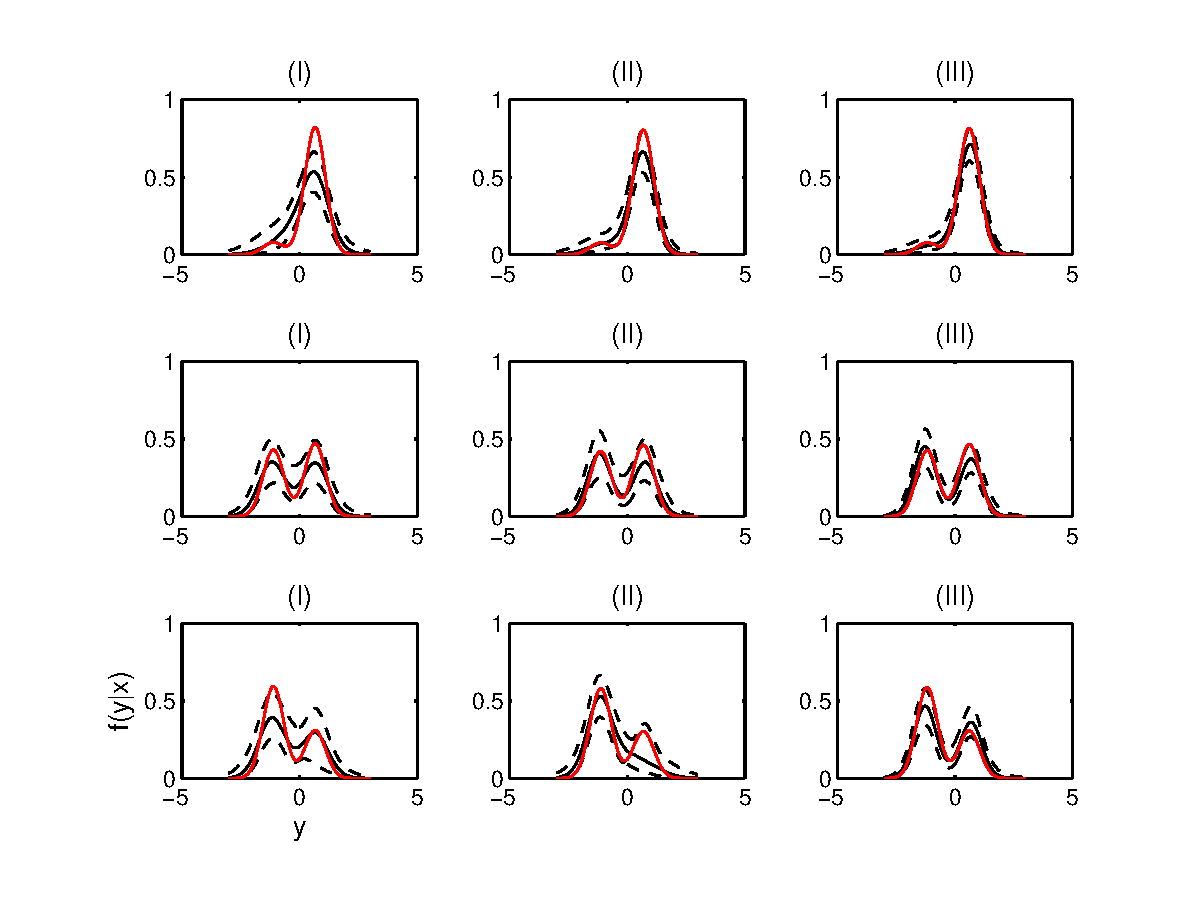
\includegraphics[width=120mm,height=100mm]{ch3_density.eps}
% 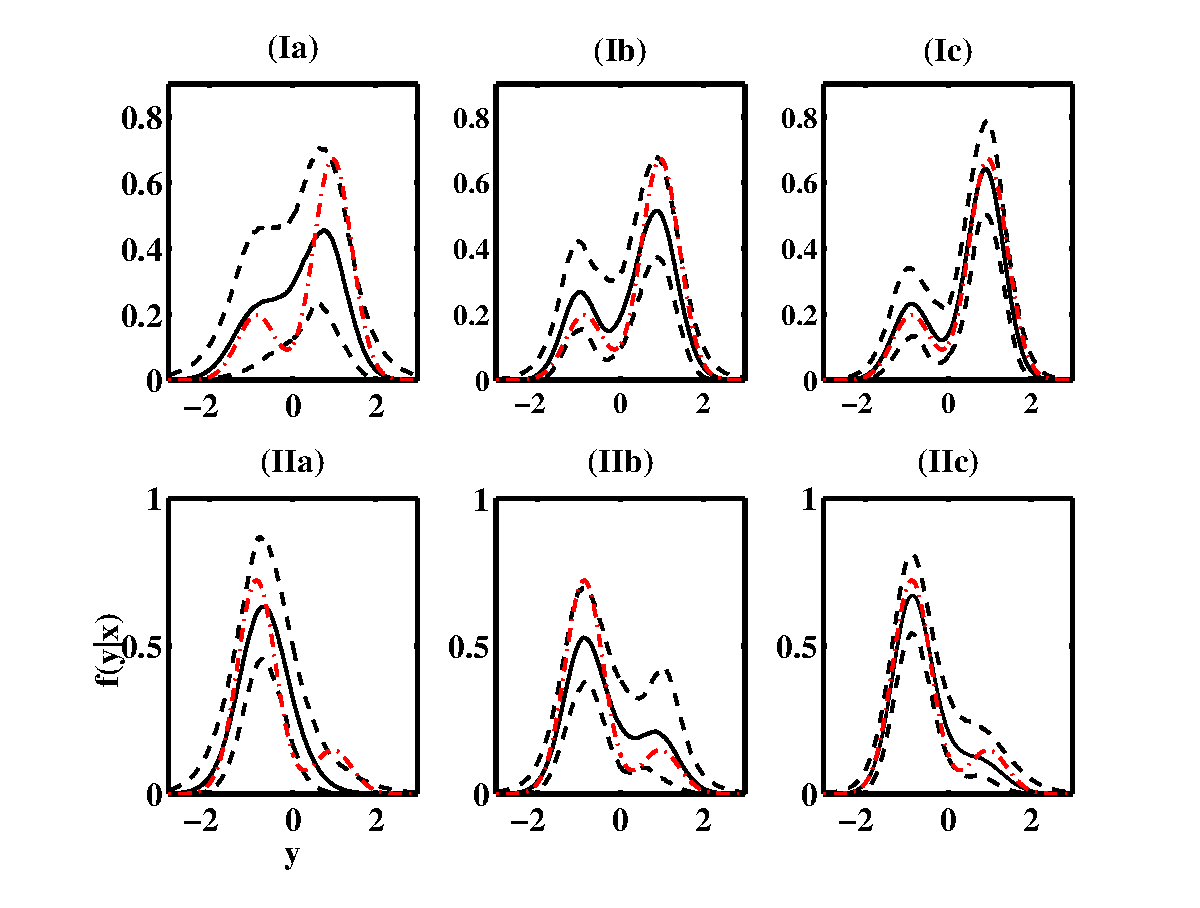
\includegraphics[width=90mm,height=80mm]{densityestimate.eps}
\caption{Illustrative example: Plot of true (red dashed-dotted line) and estimated ($50$th percentile: solid line, $2.5$th and $97.5$th percentiles: dashed lines) density for five data points $(I, II,III, IV, V)$ considering different training set size (a:100, b:200, c:300). } \label{plotDensity}
\end{figure}


%% INSERT  For each resolution level, the new observation was allocated to the set with closer center. 

\subsection{Linear lower dimensional space} \label{section:linear}

In this section, the vector of predictors was assumed to lie close to a lower dimensional plane. In practice,  predictors were modeled through a factor model as follows 

\begin{equation} x_i=\Lambda \eta_i + \epsilon_i \end{equation} 

with $\epsilon_i \sim \mc{N}(0,\Sigma_0)$, $\Sigma_0=diag(\sigma_1, \ldots, \sigma_p)$, $\Lambda$ being a $p \times r$ matrix, $\eta_i \sim \mc{N}(0,I)$ and $r\ll p$. In the first simulation scenario the response $y$ was assumed to be a function of the latent variable $\eta$ so that  the dependence between response and predictors was induced by the shared dependence on the latent factors. In practice, the pair $(y_i, x_i)$ was jointly sampled from a factor model. The loading matrix was derived as the product of a matrix with orthogonal columns and a diagonal matrix with positive elements on the diagonal, i.e. $\Lambda=\Gamma \Theta$. In particular, the columns of $\Gamma$ were uniformly sampled from the Stiefel manifold while the diagonal matrix of $\Theta$ were sampled from an inverse Gamma with shape and rate parameters $(1,4)$. In the second simulation scenario, $x$ was sampled from a factor model with sparse loading while $y$ was sampled from a normal with location and scale parameter $(1,1)$ if the first variable was positive, i.e. $x_1>0$, and from a normal with location and scale $(-1,1)$ otherwise.  In this example, the non zero elements of the loading matrix were sampled from a normal with zero mean and standard deviation $3$. In all the examples, an inverse gamma prior with parameters $(1,4)$ were utilized for $\sigma_j$ with $j=1, \ldots, p$.

Table \ref{table:linear1} and \ref{table:linear2} show mean squared errors under the proposed approach, CART and LASSO based on leave-one-out prediction. As shown in table \ref{table:linear1} and table \ref{table:linear2}, in almost all data scenario, our model is able to perform as well as or better than the model associated to the lowest mean squared error. In the first data scenario, given the linear relationship between response and predictors, Lasso performs better CART in almost all experiments. On the other hand, the non linear relationship between response and predictors assumed in the second data scenario results in better performance for CART. Table \ref{table:linear1} and figure \ref{Cpu} show the mean of CPU usage to predict a single point as a function of the number of features. In particular, CPU time is expressed in seconds and codes have been running on our workstation (Intel Core i7-2600K Quad-Core Processor memory 8192 MB).  Clearly, the proposed model scale substantially better than others to high dimensional predictors. 


\begin{figure}[h!]
\centering
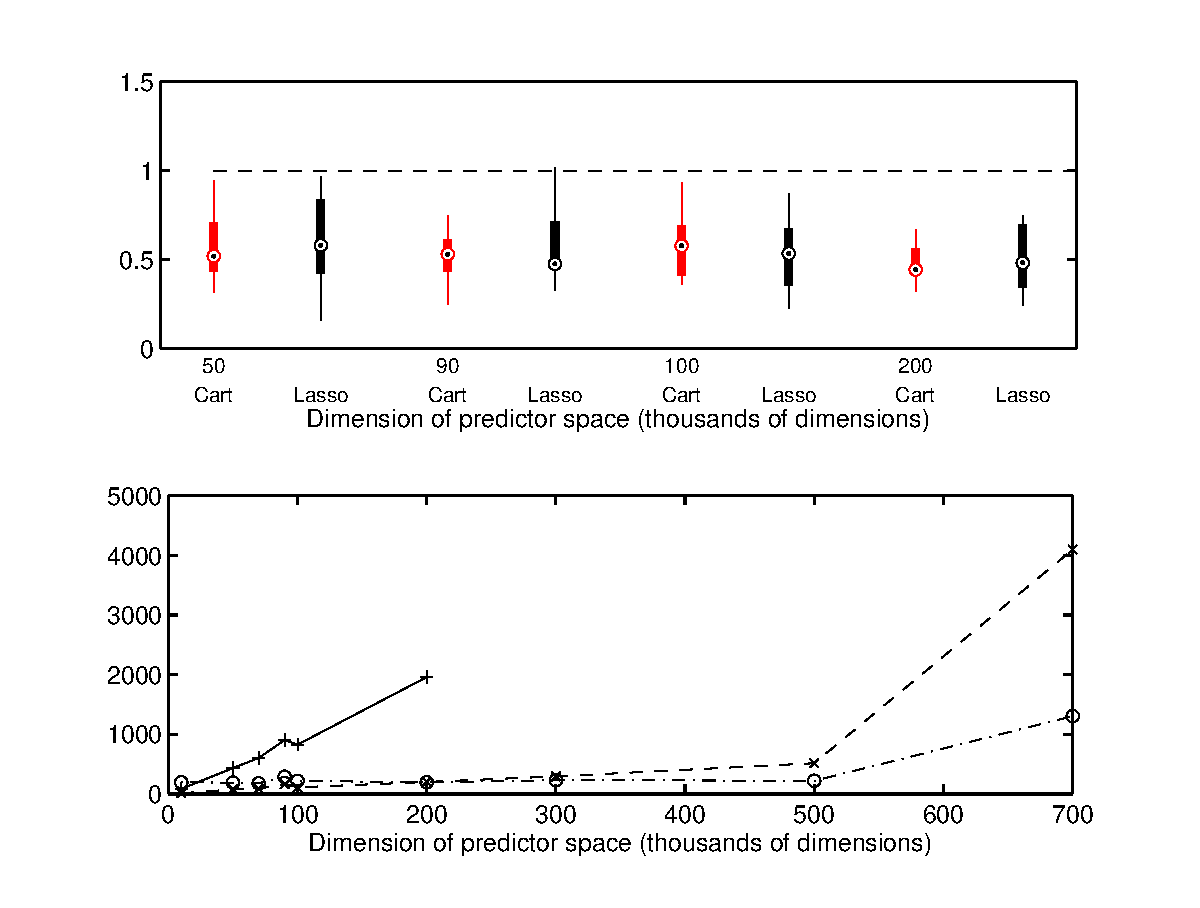
\includegraphics[width=120mm,height=80mm]{box_exp1.eps}
% 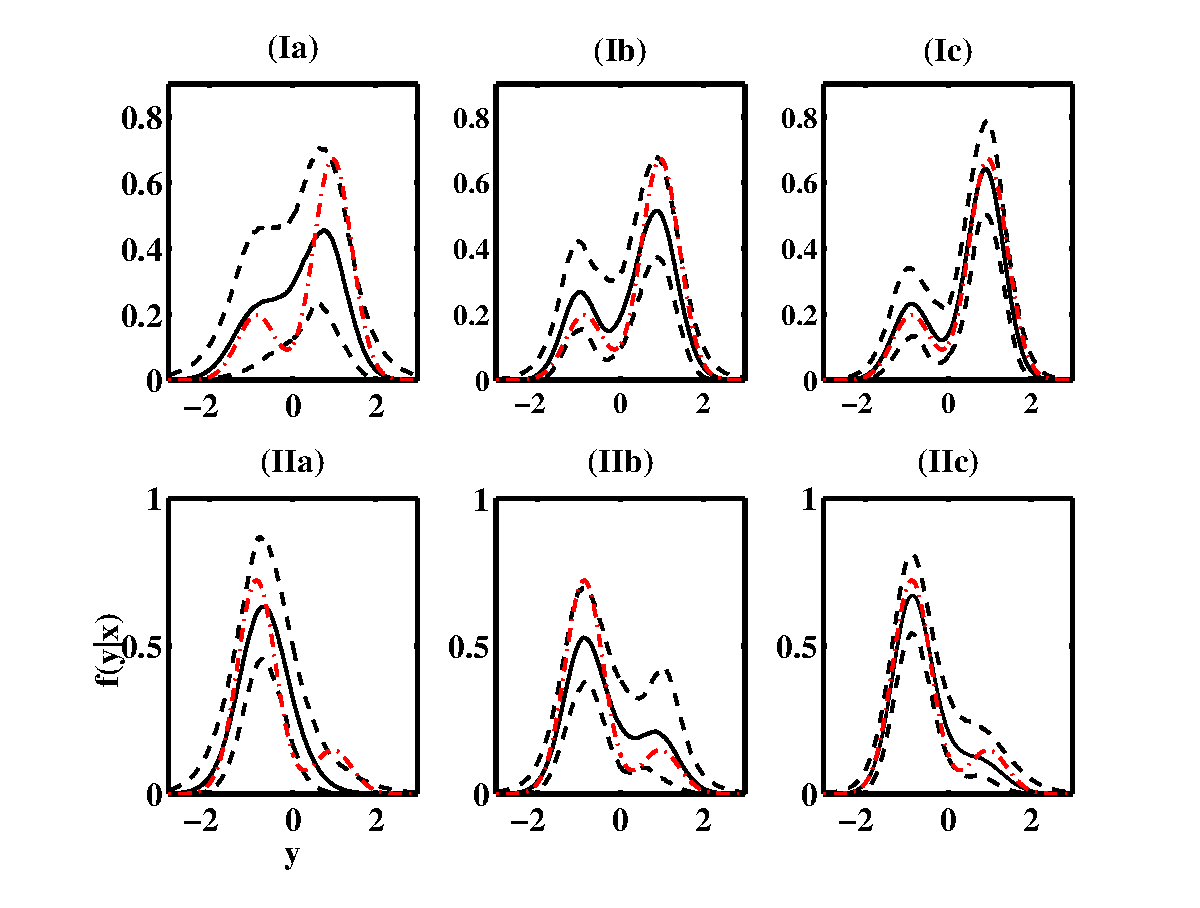
\includegraphics[width=90mm,height=80mm]{densityestimate.eps}
\caption{ } \label{boxplot:linear}
\end{figure}





\subsection{Non-Linear lower dimensional space}

In this section predictors were assumed to lie close to a lower dimensional non-linear manifold. In the first simulation study, predictors and response were jointly sampled from an $N$ components mixture of factor analyzers  so that the vector of predictors and response were assumed to lie close to $N$ lower dimensional planes. For each mixture components, the loading matrix and variances were sampled as in the first simulation scenario in \S \ref{section:linear}, while mixture weights were sampled from a Dirichlet distribution with parameter $\alpha_j=1$ for $j=1, \ldots, N$. The number of latent factors was considered to be increasing in the number of components, in practice we let the $h$th mixture component be modeled through $h$ factors. In the other simulation scenarios predictors were assumed to lie close to the Swissroll and the S-manifold (see figure \ref{manifold:nonlinear}), all two dimensional manifold embedded in $\Real^p$ while the response was sampled from a normal with mean equal to one of the coordinates of the manifold and standard deviation one.

As in \S \ref{section:linear}, the proposed model was compared in terms of computational time and predictive performance with LASSO and Cart. Table \ref{table:mfa} and \ref{table:swiss}  show computational time and mean squared errors based on leave-one-out predictions considering each of the three simulation scenario.  In particular, table \ref{table:mfa} shows the results associated to the data drawn from the mixture of factor analyzers for different number of components. In this example, given the linear relationship between predictors and response, Lasso performs better than CART. Lasso is also much more efficient than CART and performs similarly to our model for moderately high dimensional features. However, as shown in table \ref{table:mfa}, as the sample size increases the computational time associated to Lasso dramatically increases compared to our model (see $p=300,000$ for $n=100, 200, 300$). Table \ref{table:swiss} also shows that our model is associated to better predictive performance and CPU time.




\begin{figure}
\centering
\begin{tabular}{cc}
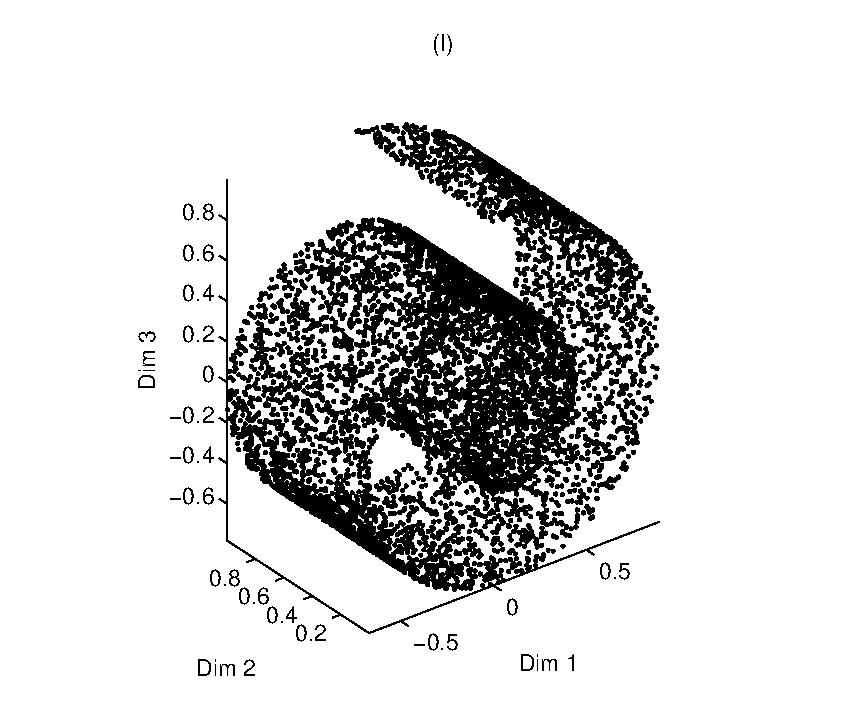
\includegraphics[width=60mm,height=50mm]{Swissroll.eps} & 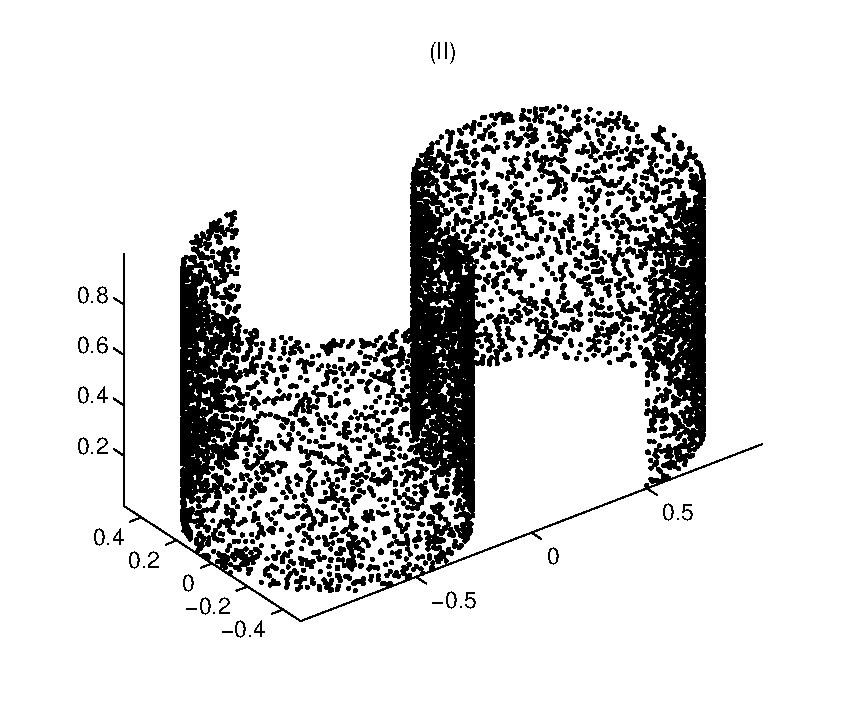
\includegraphics[width=60mm,height=50mm]{SManifold.eps}
\end{tabular}
\caption{Non-linear manifolds: Swissroll (I) and S-Manifold (II) embedded in $\mathcal{R}^3$} \label{manifold:nonlinear}
\end{figure}



\section{Real application}

We assessed the predictive performance of the proposed method on two very different neuroimaging datasets. First, we consider a structural connectome dataset collected at the Mind Research Network.  Data were collected as described in Jung et al. \cite{Jung2010}.
% ,and structural connectomes were estimated using the Magnetic Resonance Connectome Automated Pipeline \cite{MRCAP}.  
% Each of the $108$ children underwent both multimodal imaging and a battery of cognitive assessments.  
We investigated the extent to which we could predict creative (as measured via the Composite Creativity Index \cite{Arden2010}).   For each subject, we estimate a $70$ vertex undirected weighted brain-graph using the Magnetic Resonance Connectome Automated Pipeline \cite{MRCAP11} from diffusion tensor imaging data \cite{Mori2006}. We therefore let each $x_i \in \Real^p$ correspond to logarithm of each weighted edge; because our graphs are undirected and lack self-loops, we have a total of $\binom{70}{2}=2,415$ potential weighted edges.
The vector of covariates consists in the natural logarithm of the total number of connections between all pairs of cortical regions, i.e. $p=2,415$. 

The second dataset comes from a resting-state functional magnetic resonance experiment as part of the Autism Brain Imaging Data Exchange \cite{Autism}.  We selected the Yale Child Study Center for analysis.  Each brain-image was processed using the Configurable Pipepline for Analysis of Connectomes \cite{cpac}. For each subject we computed a measure of normalized power at each voxel called fALFF \cite{Zou2008}.  fALFF is a highly nonlinear transformation of the time-series data, previously demonstrated to be a reliable property of such data.  To ensure the existence of nonlinear signal relating these predictors, we let $y_i$ correspond to an estimate of overall head motion in the scanner, called mean framewise displacement (FD) computed as described in Power et al. \cite{power}.

% Our interest was predicting the head motion measurement based on $3$D brain images involving about one million of pixels. These $3$D matrices were vectorized and considered as predictors in our model. In order to reduce the dimensionality of the predictor space the data was re-processed using a brain mask and a vector of about $300,000$ predictors  was obtained.

For the analysis, all variables were normalized by subtracting the mean and dividing by the standard deviation. The same prior specification and Gibbs sampler as in \S 5 was  utilized. Table \ref{real} shows mean and variance squared error based on leave-one-out predictions. Variable $t_{T}$ is the amount of time necessary to obtain predictions for all subjects, while variables $t_M$ and $t_V$ are respectively the mean and the standard deviation of amount of time necessary to obtain one point predictions.

For the first data example, we compared our approach (multiresolution stick-breaking; MSB) to CART, LASSO and random forests. 
Table \ref{real} shows that MSB outperforms all the competitors in terms of mean square error; this is in addition to yielding an estimate of the entire conditional density for each $y_i$.  It is also significantly faster that random forests, the next closest competitor, and faster than LASSO.  For this relatively low-dimensional example, CART is reasonably fast.  

 % random forest in terms of mean squared error, and is associated to a much lower CPU time. This real data application does not involve a huge number of predictors so that computationally our model performs almost as well as LASSO and CART. However, as  shown in section 5, our model can scale substantially better than all other models to huge number of features. \\
 
 For the second data application, given the huge dimensionality of the predictor space, we were unable to get either CART or random forest to run to completion, yielding memory faults on our workstation (Intel Core i7-2600K Quad-Core Processor memory 8192 MB).  We thus only compare performance to LASSO.  As in the previous example, MSB outperforms LASSO in terms of predictive accuracy measured via mean-squared error, and significantly outperforms LASSO in terms of computational time.  
 % and the poor scalability of CART and random forest, the comparison was made only with LASSO. As shown in table \ref{real}, our approach is more efficient and accurate than LASSO in predicting the response variable. 
Figure \ref{fig:real} shows the plot of CPU time used to predict each one of the $56$ subjects involved in the experiment. The time needed to compute quantities utilized in all subject predictions was divided equally across subjects. Clearly, our approach is able to improve the computational time by up to five orders of magnitude. 


\begin{table}[t]
\caption{Real Data: Mean and standard deviations of squared error under multiscale stick-breaking (MSB), CART, Lasso and random forest (RF).}\label{real}
\vskip 0.15in
\begin{center}
\begin{small}
\begin{sc}
\begin{tabular}{llcccccccc}
\hline
data &$n$&$p$ &model&mse&$t_{T}$ & $t_{M}$ & $t_{V}$\\
\hline
(1)&108&2,415&msb &$0.56$ & $100$ & $1.1$& $0.02$\\
 &&& cart & $1.10$ & $87$ & $0.9$ &$0.01$\\
&&& LASSO & $0.63$  & $50$ & $0.40$ & $0.10$\\
&&& rf & $0.57$ &  $7,817$ & $78.2$ & $0.59$\\
\\
  (2)&56&$10e+05$&msb &$0.76$ & $690$ & $20.98$& $2.31$\\
 &&& LASSO & $1.02$  & $5,836$ & $96.18$ & $9.66$\\
\hline
\end{tabular}
\end{sc}
\end{small}
\end{center}
\vskip -0.1in
\end{table}


\nocite{langley00}



\begin{figure}[h!]
\centering
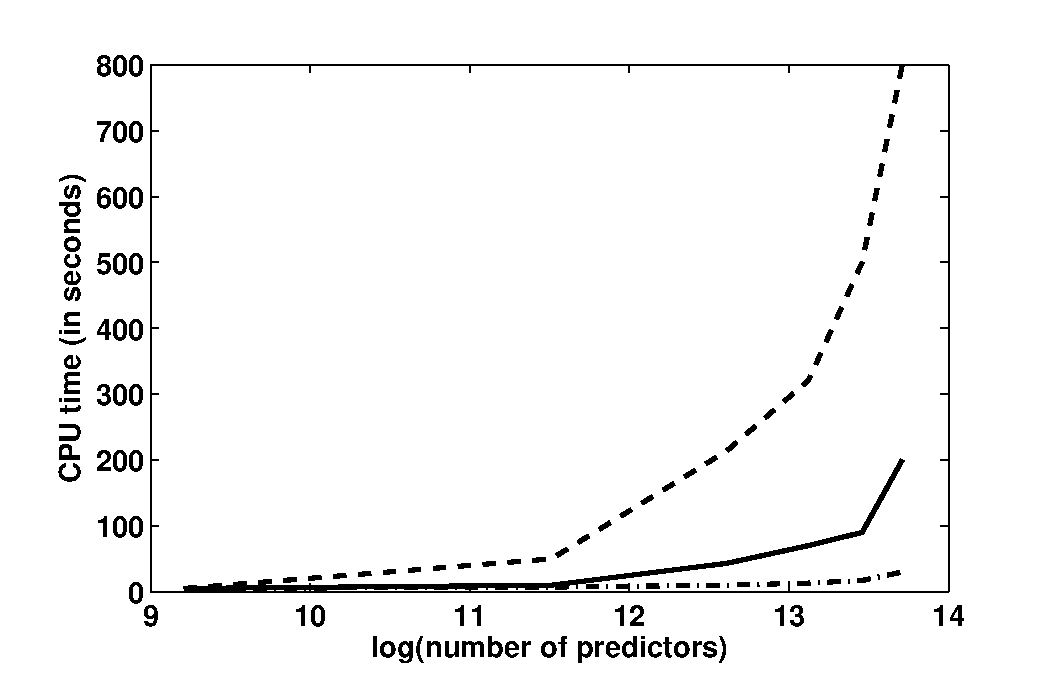
\includegraphics[width=0.8\linewidth]{plotCPU.eps}
% 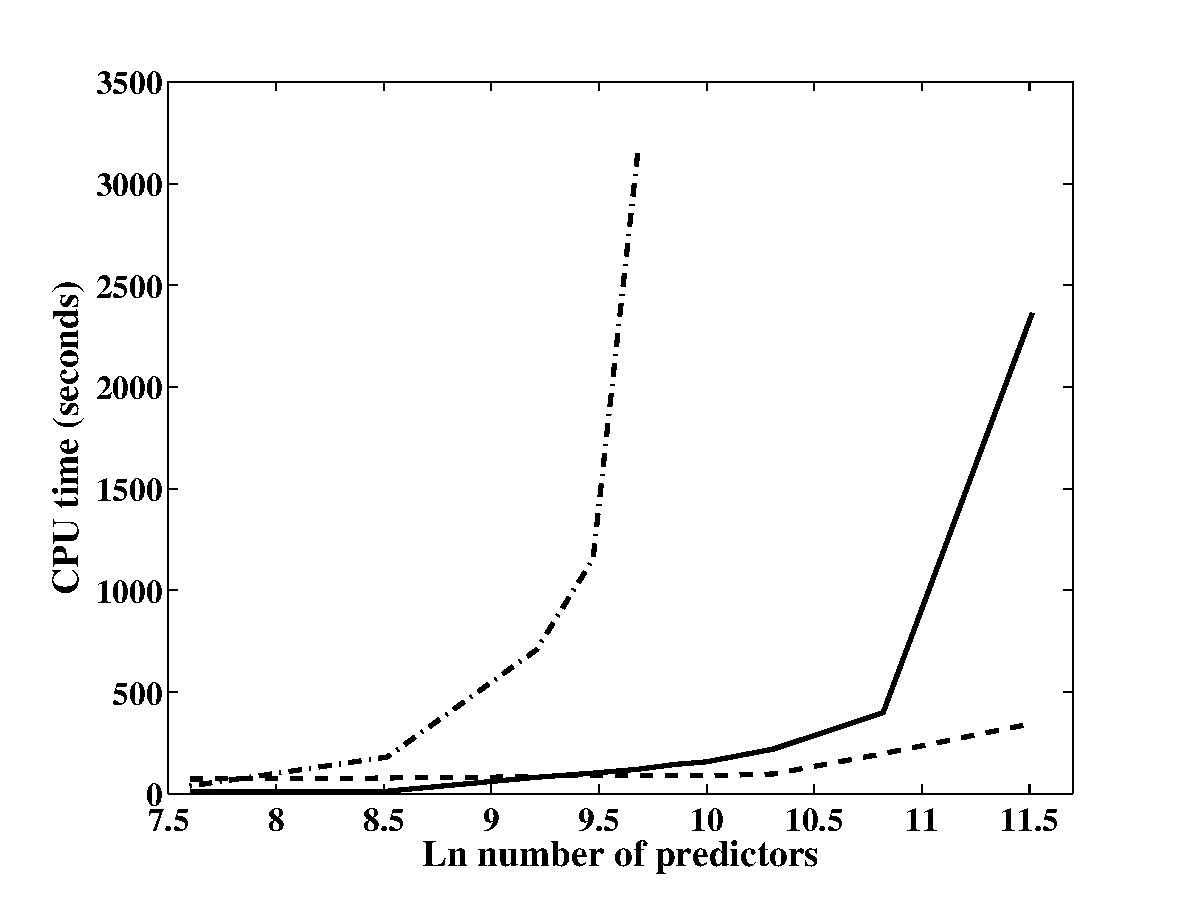
\includegraphics[width=80mm,height=45mm]{Cpu.eps}
\caption{Elapsed CPU time (in seconds) for a single point prediction based on $200$ observations for MSB (dot-dash), LASSO (solid) and CART (dash) for different number of predictors in log-scale.} \label{Cpu}
\end{figure}

\begin{figure}[h!]
\centering
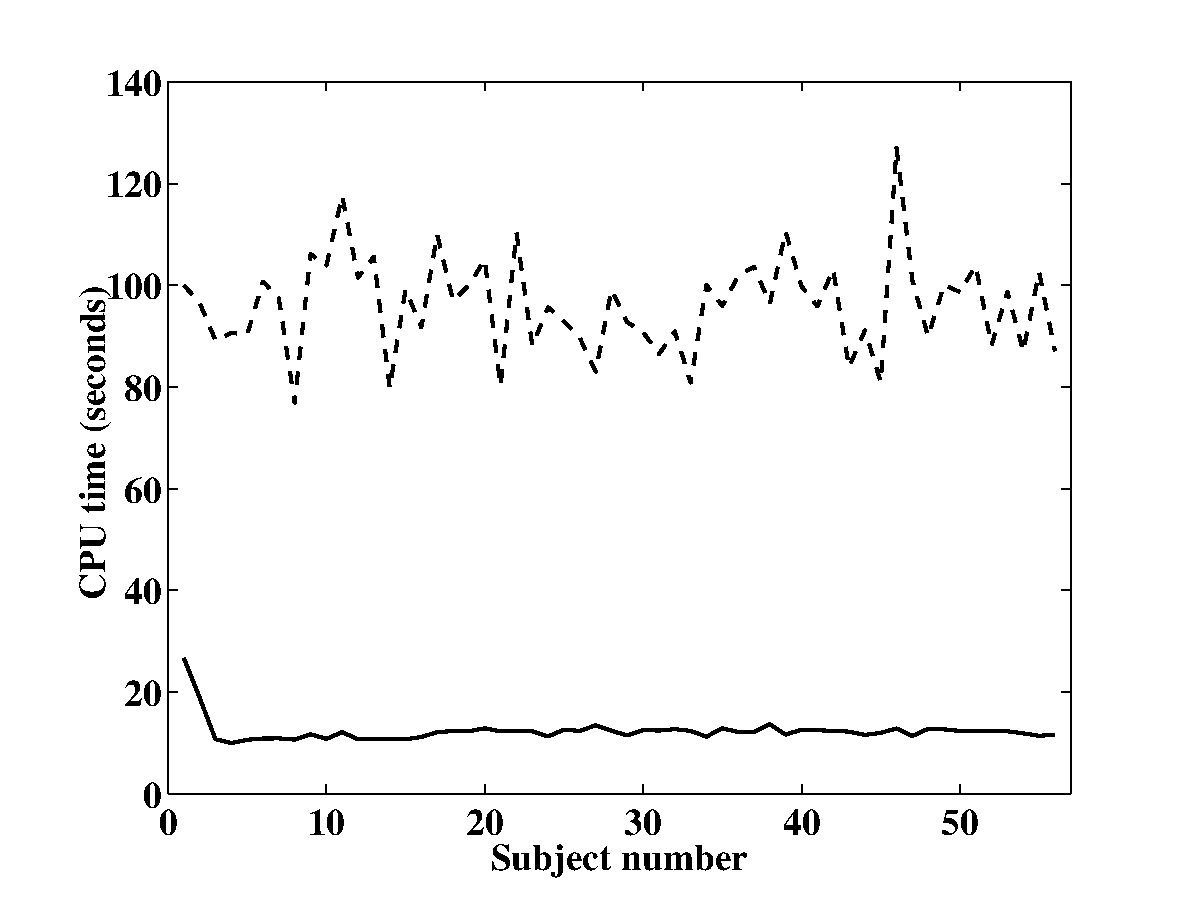
\includegraphics[width=1.0\linewidth]{Time_real2.eps}
% 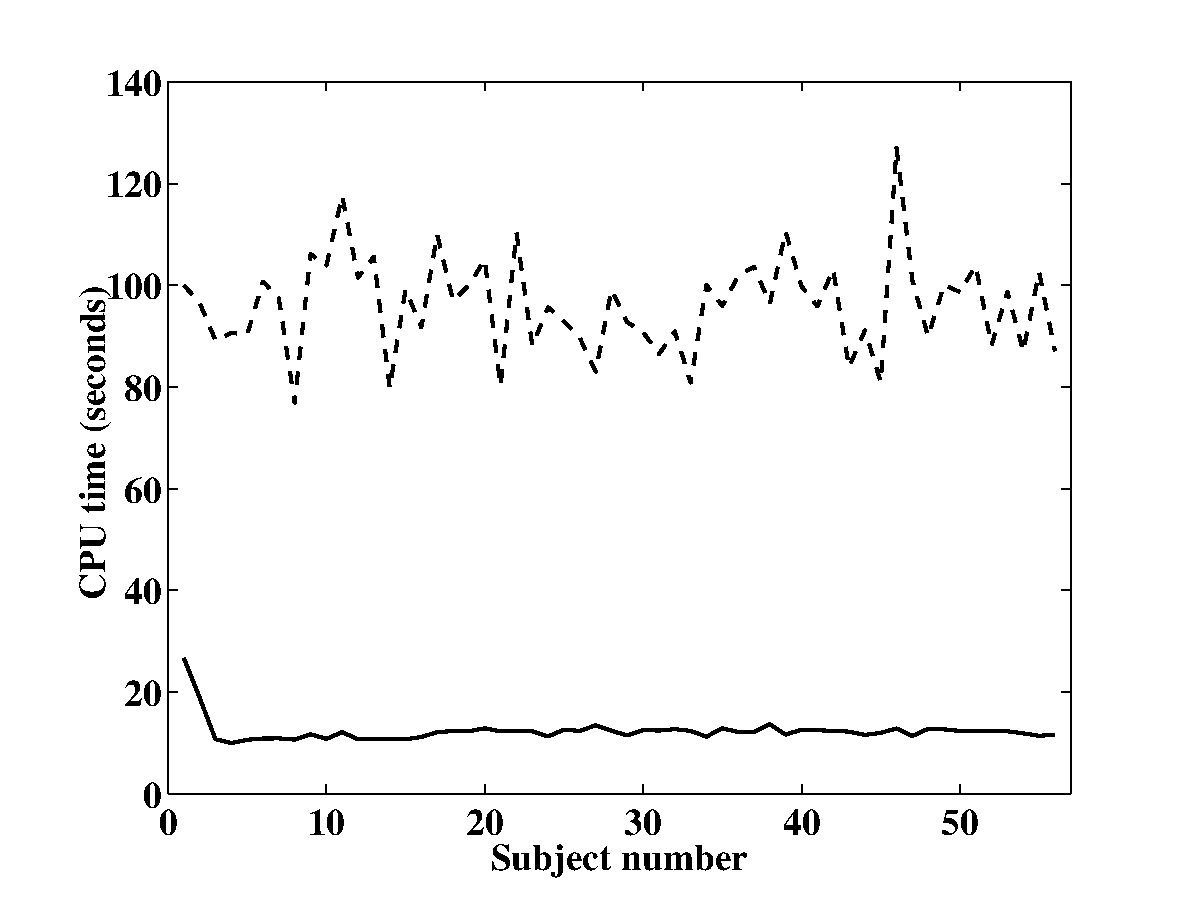
\includegraphics[width=80mm,height=40mm]{Time_real2.eps}
\caption{Plot of CPU time used to predict each one of the $56$ measurement involved in experiment (2) under MSB (solid) and LASSO (dash).} \label{fig:real}
\end{figure}

\section{Conclusion}
We have proposed a new model which should lead to substantially improved predictive and computational performance to learn the density of a target variable given a high dimensional vector of predictors. As shown the proposed two stage approach can scale substantially better than other existing algorithms to massive number of features. We have focused on Bayesian MCMC-based methods, but there are numerous interesting directions for ongoing research. Moreover, in addition to better predictive and computational performance, our methods easily extend to parallelized and distributed systems, which we will also explore in future work.


\bibliographystyle{unsrt} 
\bibliography{nipsMSB} 


\appendix
\section{Tables}

\begin{table}[t]
\caption{Linear manifold example 1: Mean and standard deviations of squared errors under multiscale stick-breaking (MSB), CART and Lasso for sample size 50 and 100 for different simulation scenarios.}\label{table:linear1}
\vskip 0.15in
\begin{center}
\begin{small}
\begin{sc}
\begin{tabular}{lllcccccc}
\hline
&&&\multicolumn{3}{c}{$r=5$}&\multicolumn{3}{c}{$r=10$}\\
$p$&$n$& & msb&cart&LASSO & msb&cart&LASSO \\
\\
\multirow{3}{*}{$10e+03$}&\multirow{3}{*}{50}&\bfoo mse\efoo&0.18&0.31&0.25&0.22&0.58&0.22\\
&&\bfoo std\efoo &0.32&0.30&0.42&0.24&0.54&0.30\\
&&\bfoo time\efoo &3&2&1&3&3&1\\

\\
\multirow{3}{*}{$10e+03$}&\multirow{3}{*}{100}&\bfoo mse\efoo&0.18&0.27&0.26&0.20&0.41&0.52\\
&&\bfoo std\efoo & 0.26&0.42&0.46&0.23&0.46&0.78\\
&&\bfoo time\efoo &5&5& 2&5&5&1\\

\\
\multirow{3}{*}{$10e+04$}&\multirow{3}{*}{50}&\bfoo mse\efoo&$0.35$&$0.45$&$0.89$&$0.16$&$0.33$&$0.20$\\
&&\bfoo std\efoo &$0.53$ &$0.77$&$1.04$&$0.21$&$0.46$&$0.31$\\
&&\bfoo time\efoo &$3$&$25$&$2$&$3$&$27$&$2$\\
\\
\multirow{3}{*}{$10e+04$}&\multirow{3}{*}{100}&\bfoo mse\efoo&$0.43$&$0.88$&$0.52$&$0.17$&$0.50$&$0.31$\\
&&\bfoo std\efoo &$0.59$ &$1.29$&$0.70$&$0.24$ &$0.75$&$0.49$\\
&&\bfoo time\efoo &$7$&$50$&$5$&$7$&$51$&$5$\\
\\
\multirow{3}{*}{$50e+04$}&\multirow{3}{*}{50}&\bfoo mse\efoo&0.11&0.16&0.15&0.83&2.26&0.92\\
&&\bfoo std\efoo&$0.15$ &0.24&0.19&1.01&2.60&3.69\\
&&\bfoo time\efoo &5&90&11&5&121&10\\


\\
\multirow{3}{*}{$50e+04$}&\multirow{3}{*}{100}&\bfoo mse\efoo&0.003&0.17&0.08&0.13&1.37&1.06\\
&&\bfoo std\efoo &0.16&0.23&0.13&1.12&1.81&1.50\\
&&\bfoo time\efoo &10&214&43&8&227&42\\

\\
\multirow{3}{*}{$70e+04$}&\multirow{3}{*}{50}&\bfoo mse\efoo&1.70&1.48&1.47&0.66&1.65&1.07\\
&&\bfoo std\efoo &2.18&2.47&1.63&0.87&1.49&0.95\\
&&\bfoo time\efoo &6&121&12&7&151&13\\

\\
\multirow{3}{*}{$50e+04$}&\multirow{3}{*}{100}&\bfoo mse\efoo&0.69&1.36&0.82&0.78&1.52&1.43\\
&&\bfoo std\efoo &0.94&1.47&1.28&1.03&1.34&2.11\\
&&\bfoo time\efoo &13&321&41&12&325&44\\

 \hline
\end{tabular}
\end{sc}
\end{small}
\end{center}
\vskip -0.1in
\end{table}


\begin{table}[t]
\caption{Linear manifold example 2: Mean and standard deviations of squared errors under multiscale stick-breaking (MSB), CART and Lasso for sample size 50 and 100}\label{table:linear2}
\vskip 0.15in
\begin{center}
\begin{small}
\begin{sc}
\begin{tabular}{lllcccccc}
\hline
&&&\multicolumn{3}{c}{$r=2$}&\multicolumn{3}{c}{$r=5$}\\
$p$&$n$& & msb&cart&LASSO & msb&cart&LASSO \\

%\multirow{3}{*}{$10^5$}&\multirow{3}{*}{100}&\bfoo mse\efoo&0.63 &0.83&0.93&0.71&0.98&0.86\\
%&&\bfoo std\efoo &0.81&0.94&1.02&0.69 &1.04&1.55\\
%&&\bfoo time\efoo &9.45 &46.15& 4.55&8.05&47.65&5.15\\
%
%\\
%\multirow{3}{*}{$20^5$}&\multirow{3}{*}{100}&\bfoo mse\efoo&0.89&0.74&1.08&0.95 &&1.15\\
%&&\bfoo std\efoo &1.50 &1.02&1.97&1.20&&1.13\\
%&&\bfoo time\efoo &7.96&102.12&8.95& 10.70&&8.75\\
%
%\\
%\multirow{3}{*}{$50^5$}&\multirow{3}{*}{100}&\bfoo mse\efoo &0.83 &&0.94\\
%&&\bfoo std\efoo &1.08&koala&1.10\\
%&&\bfoo time\efoo &9.27&&23.54\\
\\

\multirow{2}{*}{$10e+03$}&\multirow{2}{*}{100}&\bfoo mse\efoo&1.54 &1.78&2.37&0.84&1.25&1.62\\
&&\bfoo std\efoo &1.70&1.72&0.89&1.38&1.35&1.47\\


\\
\multirow{2}{*}{$50e+03$}&\multirow{2}{*}{100}&\bfoo mse\efoo&0.76&0.97&1.77&0.88&1.53&1.43\\
&&\bfoo std\efoo &1.04&1.21&3.13&1.00&1.59&2.73\\

\\

\multirow{2}{*}{$10e+04$}&\multirow{2}{*}{100}&\bfoo mse\efoo&0.77 &1.01&1.61&0.67&0.46&0.97\\
&&\bfoo std\efoo &0.94&1.13&1.85&0.82&0.61&1.16\\
%&&\bfoo time\efoo &7.69 &46.14&4.51&9.89&41.68&4.38\\
\\

\multirow{2}{*}{$20e+04$}&\multirow{2}{*}{100}&\bfoo mse\efoo&0.86&0.90&1.41&0.74&1.09&0.78\\
&&\bfoo std\efoo &1.30&1.35&1.41&0.95&1.98&0.95\\
%&&\bfoo time\efoo &8.94&& 8.86 & 9.09&&17.17\\
%
%\\
%\multirow{2}{*}{$30^5$}&\multirow{2}{*}{100}&\bfoo mse\efoo&0.78&&1.32&&&\\
%&&\bfoo std\efoo &0.60&&1.27&&&\\
\hline
\end{tabular}
\end{sc}
\end{small}
\end{center}
\vskip -0.1in
\end{table}


\begin{table}[t]
\caption{Non-linear manifold - MFA: Mean and standard deviations of squared errors under multiscale stick-breaking (MSB), CART and Lasso for sample size 50 and 100 for different simulations sampled from a mixture of factor analyzers}\label{table:mfa}
\vskip 0.15in
\begin{center}
\begin{small}
\begin{sc}
\begin{tabular}{lllcccccc}
\hline
&&&\multicolumn{3}{c}{$N=10$}&\multicolumn{3}{c}{$N=5$}\\
$p$&$n$& sim& msb&cart&LASSO & msb&cart&LASSO\\
\\
\multirow{3}{*}{$50e+03$}&\multirow{3}{*}{100}&mse&0.23&0.42&0.36&0.17&0.43&0.22\\
&&std & 0.34 &0.59&0.43&0.18&0.69&0.23\\
&&time &5&24 & 3&7&27&3\\

\\
\multirow{3}{*}{$50e+03$}&\multirow{3}{*}{200}&mse&0.23 &0.42 &0.27&0.17&0.22&0.20\\
&&std & 0.33& 0.56&0.23&0.19&0.38&0.25\\
&&time & 10 &51&8&12&56&7\\

\\
\multirow{3}{*}{$10e+04$}&\multirow{3}{*}{100}&mse&0.67&1.35&1.32&0.15&0.17&0.22\\
&&std & 1.04&2.26&1.36&0.23&0.19&0.23\\
&&time &9&47&6&6&44&5\\

\\
\multirow{3}{*}{$10e+04$}&\multirow{3}{*}{200}&mse&0.64&1.37&0.85&0.15&0.26&0.15\\
&&std &0.95 &1.77&1.29&0.24&0.42&0.24\\
&&time &15&99&15&11&89&15\\
\\
\multirow{3}{*}{$30e+04$}&\multirow{3}{*}{100}&mse& 0.26&0.39&0.31&0.63&1.40&1.01\\
&&std &0.39&0.51&0.52&0.80 &1.24& 1.46 \\
&&time &9.28&125&18&9 &145& 17\\
\\
\multirow{3}{*}{$30e+04$}&\multirow{3}{*}{200}&mse&0.25&0.47&0.26&0.63&1.17&0.92\\
&&std &0.36&0.88&0.43 & 0.80&2.11&1.04 \\
&&time &15&262&40&13&283&43\\


\\
\multirow{3}{*}{$30e+04$}&\multirow{3}{*}{300}&mse&0.25&0.30&0.30&0.62&1.42&0.70\\
&&std &0.36&0.41&0.48&0.89&1.85&0.94\\
&&time &15&463&73&16&465&89\\

\hline
\end{tabular}
\end{sc}
\end{small}
\end{center}
\vskip -0.1in
\end{table}



\begin{table}[t]
\caption{Non-linear manifold - Swissroll and S-Manifold: Mean and standard deviations of squared errors under multiscale stick-breaking (MSB), CART and Lasso for sample size 50 and 100 for different simulation scenarios.}\label{table:swiss}
\vskip 0.15in
\begin{center}
\begin{small}
\begin{sc}
\begin{tabular}{lllcccccc}
\hline
&&&\multicolumn{3}{c}{Swissroll}&\multicolumn{3}{c}{S-Manifold}\\

$p$&$n$& & msb&cart& LASSO & msb&cart& LASSO\\
\\
\multirow{3}{*}{$10e+03$}&\multirow{3}{*}{100}&mse &$0.25$&$0.46$&$0.38$&0.67&0.70&0.77\\
&&std & $0.24$ & $0.53$&$0.40$&0.76&0.80&0.85\\
&&time & 5& $5$&$1$&4 & 5 & 1 \\

\\
\multirow{3}{*}{$10e+04$}&\multirow{3}{*}{50}&mse &$0.24$&$0.44$&$0.25$&0.38&0.38&0.84\\
&&std & $0.24$ & $0.42$&$0.29$&0.40&0.35&0.80\\
&&time & 3 & $22$&$2$ &5&7&1\\

\\
\multirow{3}{*}{$10e+04$}&\multirow{3}{*}{100}&mse &$0.24$ & $0.43$&$0.17$&0.25&0.30&0.70\\
&&std & $0.26$&$0.55$&$0.22$&0.22 & 0.25 &0.50\\
&&time&$6$&$48$&$7$&7 & 50 & 7\\

\\

\multirow{3}{*}{$20e+04$}&\multirow{3}{*}{50}&mse &$0.24$&$0.67$&$0.29$&0.35&0.40&0.73\\
&&std & $0.23$ & $0.50$& $0.29$&0.22&0.30 &0.40\\
&&time & 4& $38$& $5$ & 3 & 40 & 5 \\
\\
\multirow{3}{*}{$20e+04$}&\multirow{3}{*}{100}&mse &$0.25$&$0.78$&$0.33$&0.37&0.37&0.70\\
&&std & $0.26$ & $0.74$&$0.36$&0.25&0.27&0.55\\
&&time &6 &$96$&$13$ &6&98&14\\
\\

\multirow{3}{*}{$50e+04$}&\multirow{3}{*}{50}&mse &$0.17$&$0.47$&$0.23$&0.16 &0.20&0.35\\
&&std & $0.23$ & $0.43$&$0.22$&0.20&0.19&0.40\\
&&time &$5$ &$126$&$10$ & 5 & 130 &15 \\

\\
\multirow{3}{*}{$50e+04$}&\multirow{3}{*}{100}&mse &$0.17$&$0.33$&$0.19$&0.11&0.25&0.56\\
&&std & $0.21$ &$0.46$ &$0.23$&0.14&0.20 &0.61\\
&&time &$11$ &$230$&$25$&10&254 &27\\



\hline
\end{tabular}
\end{sc}
\end{small}
\end{center}
\vskip -0.1in
\end{table}


\end{document}
